\chapter{Ricerca locale}

\paragraph{Ricerca Locale}
    Per ricerca locale si intende, a partire da una soluzione ammissibile, la ricerca di una soluzione migliore nell'intorno di essa. Si prosegue quindi a modificare la soluzione corrente, fino a quando non si riesce più a trovare una soluzione migliore. La ricerca locale è un metodo di ottimizzazione che può essere applicato a problemi di ottimizzazione.

\section{Flusso Massimo}

    \paragraph{Rete di flusso, sorgente, pozzo, capacità}
        Una rete di flusso è costituita da un grafo orientato, un nodo sorgente, un nodo pozzo e la funzione di capacità. La sorgente è il nodo da cui partono i flussi, mentre il pozzo è il nodo in cui i flussi si accumulano. La funzione di capacità definisce la massima quantità di flusso che può passare attraverso ciascun arco della rete.\newline
        Si assume che per ogni nodo $x\in V$ esista un cammino $s \rightsquigarrow x$ e un cammino $x \rightsquigarrow t$ da $s$ a $t$ che passi per $x$. I nodi $s$ e $t$ sono i nodi sorgente e pozzo, rispettivamente.
    \paragraph{Flusso}
        Un flusso è una funzione che associa a ciascun arco della rete un valore reale, che rappresenta la quantità di flusso che passa attraverso l'arco. Il flusso deve rispettare le seguenti condizioni:
        \begin{itemize}
            \item La capacità di ciascun arco non può essere superata.
            \item Deve essere antisimmetrica cioè se $f(u,v)$ è il flusso che va da $u$ a $v$, allora $f(v,u) = -f(u,v)$.
            \item Il flusso deve essere conservato, cioè ($\forall x \in V-\{s,t\}, \sum_{y \in V} f(x,y) = 0$).
        \end{itemize}
        viene allora definito il valore del flusso come la somma dei flussi in uscita dalla sorgente, cioè $\displaystyle |f| = \sum_{(s,x)\in E} f(s,x)$.
        Il flusso massimo è il flusso che massimizza il valore del flusso, cioè il flusso che massimizza la somma dei flussi in uscita dalla sorgente. 
    \subsubsection{Algoritmo delle reti residue}
        Per calcolare il flusso massimo in una rete di flusso si può utilizzare l'algoritmo delle reti residue. Questo prevede la memorizzazione di un flusso (inizialmente nullo) e la ripetizione delle seguenti operazioni:
        \begin{enumerate}
            \item Si rimuove il flusso attuale dalla rete di flusso, ottenendo una \textbf{rete residua}.
            \item Si cerca un flusso $g$ all'interno della rete residua
            \item Si aggiunge il flusso $g$ alla rete di flusso, ottenendo un nuovo flusso.
        \end{enumerate}
        viene ripetuto questo processo fino a quando non si riesce più a trovare un flusso $g$ all'interno della rete residua.\newline
        Per far funzionare questo algoritmo è necessario definire ``capacità residua'' e ``rete residua''. La capacità residua di un flusso $f$ in una rete di flusso $G$ è definita come:
        $$
            \forall x,y\in V, c_f(x,y) = c(x,y) - f(x,y)
        $$
        una rete residua è una rete di flusso in cui la capacità di ciascun arco è data dalla capacità residua del flusso $f$.
        \begin{theorem}
            Se $f$ è un flusso in $G$ e $g$ è un flusso in $G_f$, allora $f+g$ è un flusso in $G$.
        \end{theorem}
        \begin{proof}
            Rispetta la conservazione $\forall x\in V-\{s,t\}$ infatti:
            \begin{align*}
                \sum_{y\in V} (f+g)(x,y) &= \sum_{y\in V} (f(x,y) + g(x,y)) \\
                &= \sum_{y\in V} f(x,y) + \sum_{y\in V} g(x,y) \\
                &= 0 + 0 \\
                &= 0
            \end{align*}
            Rispetta la antisimmetria $\forall x,y\in V$:
            \begin{align*}
                f(x,y) + g(x,y) &= -(f(y,x) + g(y,x)) \\
                &= -(f(y,x) + g(y,x)) \\
                (f+g)(x,y) &= -(f+g)(y,x)
            \end{align*}
            Rispetta la capacità $\forall x,y\in V$:
            \begin{align*}
                g(x,y) &\leq c_f(x,y) \\
                f(x,y) + g(x,y) &\leq c_f(x,y) + f(x,y) \\
                (f+g)(x,y) &\leq c(x,y) - f(x,y) + f(x,y) \\
                (f+g)(x,y) &\leq c(x,y)
            \end{align*}
            Quindi $f+g$ è un flusso in $G$.
        \end{proof}
        Come cerchiamo però un flusso $g$ all'interno della rete residua? Si prende l'arco con la minore capacità residua e si cerca un cammino da $s$ a $t$ passante per quell'arco. Se non esiste un cammino da $s$ a $t$ allora non esiste un flusso $g$ all'interno della rete residua. Se esiste un cammino da $s$ a $t$ passante per quell'arco, si può calcolare il flusso $g$ come la capacità residua dell'arco. Si può quindi aggiungere il flusso $g$ alla rete di flusso, ottenendo un nuovo flusso.
        \begin{algorithm}
            \caption{\Int[][] \textsc{maxFlow}(\Graph G, \Node s, \Node t, \Int[][] c)}
            \label{alg:maxFlow}
            \begin{algorithmic}
                \State $\Int[][] f \gets \New \Int[][]$
                \State $\Int[][] g \gets \New \Int[][]$
                \State $\Int[][] c_f \gets \New \Int[][]$
                \ForEach{$(x,y)\in G.V()$}
                    \State $c_f[x][y] \gets c[x][y]$
                    \State $f[x][y] \gets 0$
                \EndFor
                \While{$g = f_0$}
                    \State $g \gets$ flusso aumentante r oppure $f_0$
                    \ForEach{$(x,y)\in g.V()$}
                        \State $c_f[x][y] \gets c_f[x][y] - g[x][y]$
                        \State $f[x][y] \gets f[x][y] + g[x][y]$
                    \EndFor
                \EndWhile
                \State \Return $f$
            \end{algorithmic}
        \end{algorithm}
        Prima di passare alla dimostrazione della correttezza dell'algoritmo, è necessario definire il concetto di \textbf{taglio}, che è un sottoinsieme di archi della rete di flusso che separa la sorgente dal pozzo. Un taglio è definito come un insieme di archi $(x,y)$ tale che $x$ è raggiungibile da $s$ e $y$ non è raggiungibile da $t$. Il valore del taglio è dato dalla somma delle capacità degli archi del taglio. La capacità del taglio è definita come la somma delle capacità degli archi del taglio. 
        \begin{theorem}
            Dato un flusso $f$ ed un taglio ($S,T$) la quantità di flusso $F_f(S,T)$ che attraversa il taglio è uguale a $|f|$.
        \end{theorem}
        \begin{proof}
            La quantità di flusso $F_f(S,T)$ che attraversa il taglio è data dalla somma dei flussi in uscita da $S$ e in entrata in $T$ ovvero:
            \begin{align*}
                F_f(S,T) &= \sum_{x\in S,y\in T} f(x,y) \\
                &= \sum_{x\in S,y\in V} f(x,y) - \underbrace{\sum_{x\in S,y\in S} f(x,y)}_{\text{per antisimmetria }= 0} \\
                &= \sum_{x\in S,y\in V} f(x,y)\\
                &= \sum_{x\in S-\{s\},y\in V} f(x,y) + \sum_{y\in V} f(s,y) & s\in S \\
                &= \sum_{x\in S-\{s\}}\sum_{y\in V} f(x,y) + \sum_{y\in V} f(s,y) \\
                &= \sum_{x\in S-\{s\}} 0 + \sum_{y\in V} f(s,y) & \text{per conservazione } \\
                &= \sum_{y\in V} f(s,y) = |f| & \text{per definizione di flusso}
            \end{align*}
        \end{proof}
        \begin{theorem}
            Il flusso massimo è limitato superiormente dalla capacità del taglio minimo, ovvero il taglio la cui capacità è minima tra tutti i tagli possibili.
        \end{theorem}
        \begin{proof}
            Nessun flusso attraverso ad un taglio supera la capacità del flusso ($\forall f:F_f(S,T) < c(S,T)$ $\forall (S,T)$ taglio di $V$).
            \begin{align*}
                \forall f:F_f(S,T) = \sum_{x\in S,y\in T} f(x,y) \leq \sum_{x\in S,y\in T} c(x,y) = C(S,T) 
            \end{align*}
            Ciò vale per il vincolo sulla capacità del flusso, inoltre vale anche il contrario, nessun flusso attraverso un taglio supera la capacità del taglio ($\forall f:F_f(S,T) < C(S,T)$ $\forall (S,T)$ taglio di $V$). Il che ci porta a dire che il flusso che attraversa il taglio è uguale al valore del flusso massimo, quindi il valore del flusso è limitato superiormente dalla capacità del taglio minimo.
        \end{proof}
        \begin{theorem}
            Le seguenti tre affermazioni sono equivalenti:
            \begin{enumerate}
                \item $f$ è un flusso massimo
                \item non esiste alcun cammino da $s$ a $t$ nella rete residua $G_f$
                \item esiste un taglio minimo $(S,T)$ tale che $C(S,T) = |f|$
            \end{enumerate}
        \end{theorem}
        \begin{proof}
            \begin{enumerate}
                \item[$1\implies 2$] Se esistesse un cammino aumentante, il flusso potrebbe essere aumentato, quindi non sarebbe massimo.
                \item[$2\implies 3$] Poiché non esiste nessun cammino aumentante nella rete residua, allora non esiste nessun cammino da $s$ a $t$ nella rete residua. Considerando $S$ l'insieme dei vertici raggiungibili da $s$ nella rete residua, allora $T=V-S$. Poiché non esiste alcun cammino da $s$ a $t$ nella rete residua, allora dato che $s\in S$ e $t\in T$, allora $(S,T)$ è un taglio. Dato che $t$ non è raggiungibile da $s$, allora tutti gli archi $(x,y)$ con $x\in S$ e $y\in T$ sono saturi. Per il lemma del flusso di un taglio $|f| = \sum_{x\in S,y\in T} f(x,y) = \sum_{x\in S,y\in T} c(x,y) = C(S,T)$.
                \item[$3\implies 1$] Poiché per un qualsiasi flusso $f$ e un qualsiasi taglio $(S,T)$ vale $|f| \leq C(S,T)$, allora se esiste un taglio minimo $(S,T)$ tale che $C(S,T) = |f|$, allora $f$ è un flusso massimo.
            \end{enumerate}
        \end{proof}
    \subsubsection{Complessità}
        La complessità dell'algoritmo delle reti residue di Ford-Fulkerson è $O((V+E)|f*|)$ per la memorizzazione con lista e $O(V^2|f*|)$ per la memorizzazione con matrice. Questo in quanto l'algoritmo parte da un flusso nullo e ogni incremento del flusso aumenta il flusso di un'unità almeno. Dato che ogni ricerca di un cammino da $s$ a $t$ nella rete residua richiede $O(V+E)$ tempo o $O(V^2)$ tempo, a seconda della rappresentazione della rete, inoltre la somma di due flussi può essere calcolata in $O(V+E)$ tempo o $O(V^2)$ tempo, quindi la complessità dell'algoritmo è $O((V+E)|f*|)$ o $O(V^2|f*|)$.\newline
        Per l'algoritmo di Edmonds-Karp, che utilizza la ricerca in ampiezza per trovare il cammino aumentante, la complessità è $O(VE^2)$, questo è dimostrabile:
        \begin{theorem}
            L'algoritmo di Edmonds-Karp ha complessità $O(VE^2)$.
        \end{theorem}
        \begin{proof}
            Dato che vengono eseguiti al massimo $O(VE)$ aumenti di flusso ognuno dei quali richiede una visita in ampiezza $O(V+E)$ tempo allora la complessità è $O(VE(V+E))$. In quanto il numero di archi è limitato superiormente da $E=\Omega(V)$ dato che ogni nodo diverso da sorgente e pozzo ha almeno un arco in entrata e uno in uscita, quindi $O(VE^2)$.
        \end{proof}
        \begin{theorem}[Lemma - Monotonia]
            Sia $\delta_f(s,x)$ la distanza minima tra $s$ e $x$ nella rete residua $G_f$. Sia $f'=f+g$ un flusso nella rete iniziale, con $g$ flusso non nullo. Allora $\delta_{f'}(s,x) \geq \delta_f(s,x)$.
        \end{theorem}
        \begin{proof}
            Quando viene aumentato il flusso $g$ nella rete residua, alcuni archi della rete residua vengono saturati, quindi dato che questi archi venivano usati nella ricerca del cammino minimo (\texttt{BFS}), la distanza minima tra $s$ e $x$ aumenta.
        \end{proof}
        \begin{theorem}[Lemma - Aumenti di flusso]
            Il numero totale di aumenti di flusso secondo l'algoritmo di Edmonds-Karp è al massimo $O(VE)$.
        \end{theorem}
        \begin{proof}
            Partendo dalla rete residua $G_f$ e considerando un cammino aumentante $C$ allora esiste un arco critico $(x,y)$ in $C$ se \begin{align*}
                c_f(x,y) = \min_{u,v\in C}\{c_f(u,v)\}
            \end{align*}
            In ogni cammino esiste almeno un arco critico ed una volta che questo viene aggiunto al flusso, non può più essere utilizzato in un altro cammino aumentante.\newline
            Visto che i cammini aumentanti sono minimi allora $\delta_f(s,y) = \delta_{f}(s,x)+1$ dunque l'arco $(x,y)$ comparirà nuovamente nella rete di flusso solo se l'arco inverso $(y,x)$ viene usato all'interno di un cammino aumentante, consideriamo il flusso $g$ dove $(y,x)$ è un arco allora $\delta_{g}(s,x) = \delta_{f}(s,y)+1$ per il lemma di monotonia $\delta_{g}(s,y)\geq \delta_{f}(s,y)$ quindi \begin{align*}
                \delta_{g}(s,x) =& \delta_{g}(s,y)+1\\
                \geq & \delta_{f}(s,y)+1\\
                =& \delta_{f}(s,x)+2
            \end{align*}
            Quindi da quando l'arco $(x,y)$ è stato critico alla volta nella quale questo può tornare ad essere critico, il cammino minimo si è allungato di almeno $2$ passi, dato che la lunghezza massima fino al nodo $x$ è $V-2$ (sottraiamo gli archi $(x,y)$ e $(y,t)$ che sono gli ultimi due al massimo prima di $t$) quindi un arco pul diventare critico al massimo $\frac{V-2}2 = \frac{V}{2}-1$ volte.\newline
            Dato che ci sono $O(E)$ archi che possono diventare critici, il numero totale di aumenti di flusso è al massimo $O(VE)$.
        \end{proof}
        \begin{table}
            \centering
            \begin{tabular}{|c|c|c|}
                \hline
                \textbf{Algoritmo} & \textbf{Complessità} & \textbf{Note} \\
                \hline
                Ford-Fulkerson & $O((V+E)|f*|)$ & Converge con valori razionali \\
                \hline
                Edmonds-Karp & $O(VE^2)$ & Si basa su \texttt{BFS} \\
                \hline
                \dots & \dots & \dots \\
                \hline
            \end{tabular}
        \end{table}

\section{Abbinamento massimo nei grafi bipartiti}
    Il problema assume una natura reale se si considera di dover assegnare i compiti da un insieme $J$ contenete $n$ lavori ad un insieme $W$ contenente $m$ lavoratori. Ogni lavoro può essere assegnato a più lavoratori e ogni lavoratore può essere assegnato a più lavori. Si vuole quindi ottenere una relazione $R\subseteq J\times W $ tale che $(j,w)\in R$ se il lavoro $j$ può essere assegnato al lavoratore $w$. Allora il più grande sottoinsieme di output $O\subseteq R$ tale che: ogni job venga assegnato a più di un lavoratore e ogni lavoratore venga assegnato a più di un lavoro. Ciò si traduce in una rete di flusso in cui i lavori e i lavoratori sono i nodi collegati dalla relazione $R$ esiste una sorgente comune $s$ connessa a tutti i lavoratori e un pozzo $t$ connesso a tutti i lavori. La capacità di ogni arco è $1$.
    \begin{figure}[H]
        \centering
        \begin{subfigure}{0.45\textwidth}
            \centering
            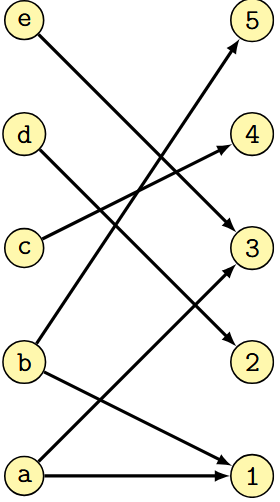
\includegraphics[scale=0.55]{16/graphBipartito.png}
            \caption{Esempio di grafo bipartito}
        \end{subfigure}
        \begin{subfigure}{0.45\textwidth}
            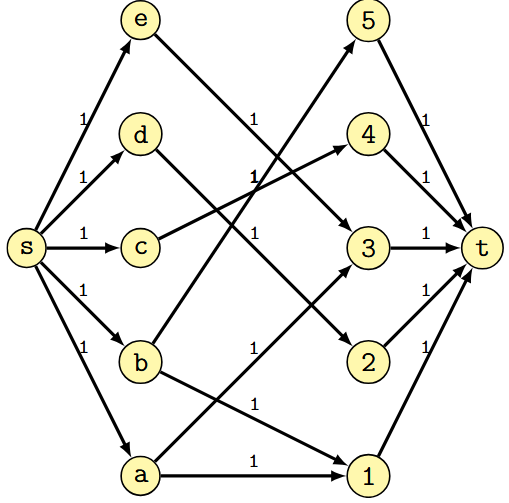
\includegraphics[width=\textwidth]{16/flussoGraphBipartito.png}
            \caption{Esempio di grafo bipartito tradotto in rete di flusso}
        \end{subfigure}
        \caption{Esempio di traduzione da grafo bipartito a rete di flusso}
    \end{figure}